\documentclass[10pt,a4paper]{article}
  \usepackage{pythontex}
  \usepackage[cm]{fullpage}
  \usepackage{newtxtext}
  \usepackage{newtxmath}
  \usepackage[
backend=biber,
style=numeric,
]{biblatex}
  \usepackage[hidelinks]{hyperref}
  \usepackage{graphicx}
  
\begin{document}
\begin{titlepage}
	\centering
	{\scshape\LARGE Web Science (H) COMPSCI4077 \par}
	\vspace{1cm}
	{\scshape\Large Network based Social Media Analytics\par}
	\vspace{1.5cm}
	{\huge\bfseries Scott Brown - 2305539B \par}
	\vspace{2cm}
	{\Large Sourcecode\par}
	{\Large \url{https://github.com/BlueLinks/WebScience-WebCrawler}\par}
	\vspace{2cm}
	{\Large Data\par}
	{\Large \url{https://github.com/BlueLinks/WebScience-WebCrawler/blob/master/all_tweets.json}\par}
	\vfill

% Bottom of the page
	{\large \today\par}
	
\end{titlepage}

\section{Introduction}
\subsection*{a.}
For my analytics I have written 5 python scripts. \\

	\verb|get_tweet_data.py| - This script uses lists 'keywords' and 'users' to filter a stream of twitter data and insert the raw tweet json into a mongoDB collection \verb|TwitterStream.all_tweets|. To use this script your twitter api access keys must be contained in a file \verb|keys.txt|. Each key must be placed on a newline with no extra characters in the order \verb|consumer_key| > \verb|consumer_secret| >\verb|access_token| and \verb|access_token_secret| with \verb|consumer_key| being on the top line and \verb|access_token_secret| being on the bottom line. \\
	
	\verb|cluster_text.py| - Simple script to find all tweets in a collection and cluster all the text in the '\verb|text|' field into k categories and print the top 10 words used \\
	
	\verb|cluster.py| - Similar to the \verb|cluster_text.py| script but instead of just the text this script extracts usernames and hashtags. To build this and the \verb|cluster_text.py| scripts I used this stack overflow question as a reference \url{https://stackoverflow.com/questions/27889873/clustering-text-documents-using-scikit-learn-kmeans-in-python} \\
	
	\verb|user_interactions.py| - This is the most complex of the three and uses the networkx and matplot libraries to draw the user interaction graphs. Lines '\verb|63|', '\verb|65|' , '\verb|67|', and '\verb|69|' can be commented in and out to control which interactions are graphed.
	\begin{verbatim}
    # Add Mentions
    interactions.add((row["user_mentions_id"], row["user_mentions_screen_name"]))
    # Add Retweets
    interactions.add((row["retweeted_id"], row["retweeted_screen_name"]))
    # Add replies
    interactions.add((row["in_reply_to_user_id"], row["in_reply_to_screen_name"]))
    # Add quotes
    interactions.add((row["quoted_id"], row["quoted_screen_name"]))
	\end{verbatim}
	I used this medium article \url{https://medium.com/future-vision/visualizing-twitter-interactions-with-networkx-a391da239af5} as a reference while building this script \\
	
	\verb|get_hashtags.py| - This script is used to get the hashtag information from the \verb|TwitterStream.all_tweets| collection in a format that is readable by \url{https://www.cortext.net} to produce graphs for the hashtag data.
	
	
\subsection*{b. } 
Data was collected for the initial 1\% stream on Tuesday the 3rd of March at 3pm and data collected using the more specific rest probes was collected on Monday the 9th of March at 6pm. To collect as much data as possible for the initial stream, generic keywords found at \url{https://techland.time.com/2009/06/08/the-500-most-frequently-used-words-on-twitter/} were used 

\section{Data crawl}
	\subsection*{a. 1\% of Data}
	I used the tweepy library to construct my twitter crawler and pymongo to connect to the local mongoDB database
	\begin{verbatim}
    def on_data(self, data):
        if (time.time() - self.start_time) < self.limit:
            # Load the Tweet into the variable "tweet"
            tweet = json.loads(data)
            try:
                all_collection.insert_one(tweet)
                return True
            except:
                # This is a duplicate
                self.duplicates += 1
                print("Duplicates so far: %d" % self.duplicates)
        else:
            # Times Up
            return False
	\end{verbatim}
	This code is called whenever the stream receives a tweet. When initialising the listener there is an option to specify a time limit in minutes (defaults to 1hr). The full raw json is inserted into the collection \verb|TwitterStream.all_tweets| and a try/except structure is used to avoid duplicates and track the number of them which is printed at the end of execution.
	From the first initial stream I identified that there was a noticeable trend with the current presidential election in the US \\ \\
	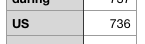
\includegraphics[scale=1]{images/US.png}
	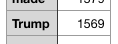
\includegraphics[scale=1]{images/trump.png} 
	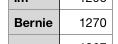
\includegraphics[scale=1]{images/bernie.png}
	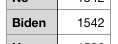
\includegraphics[scale=1]{images/biden.png} 
	
	\subsection*{b. Enhancing the crawler} 
	After deciding on looking at the presidential election race I decided to use keywords
	\begin{verbatim}
	keywords = ['trump','biden','republican','democrat',"bernie",'bernie sanders','sanders','joe',
	'donald','presidential election','@realDonaldTrump','#PresidentialRace2020','#PresidentialPrimary',
	'@BernieSanders','Bill','@JoeBiden','@SenSanders','#2020election']
	\end{verbatim}
	and users  @realDonaldTrump, @BernieSanders, and @JoeBiden
	\begin{verbatim}
	users = ['25073877','216776631', '939091']
	\end{verbatim}
	I configured the stream as follows
	\begin{verbatim}
	stream.filter(follow=users, track=keywords, languages=["en"],is_async=True)
	\end{verbatim}
	
\section{Grouping of tweets}
	\subsection*{a. Method for grouping}
	For the grouping of the tweets I wrote a python script '\verb|cluster.py|' to load all the data into a dictionary containing usernames and the full text of the tweets and used the sklearn library to vectorise and cluster the dictionary.
	I chose to cluster into 8 groups as that gave a wide spread of information and use the cluster centres to identify key records and because I used KMeans, all the clusters are of equal size.
	\subsection*{b. Method for Username and Hashtag identification}
	To indentify key usernames and hashtags from groups I used regular expressions to extract usernames and hashtags and then used a collections.Counter object to count occurrences. \\
	For example:
	
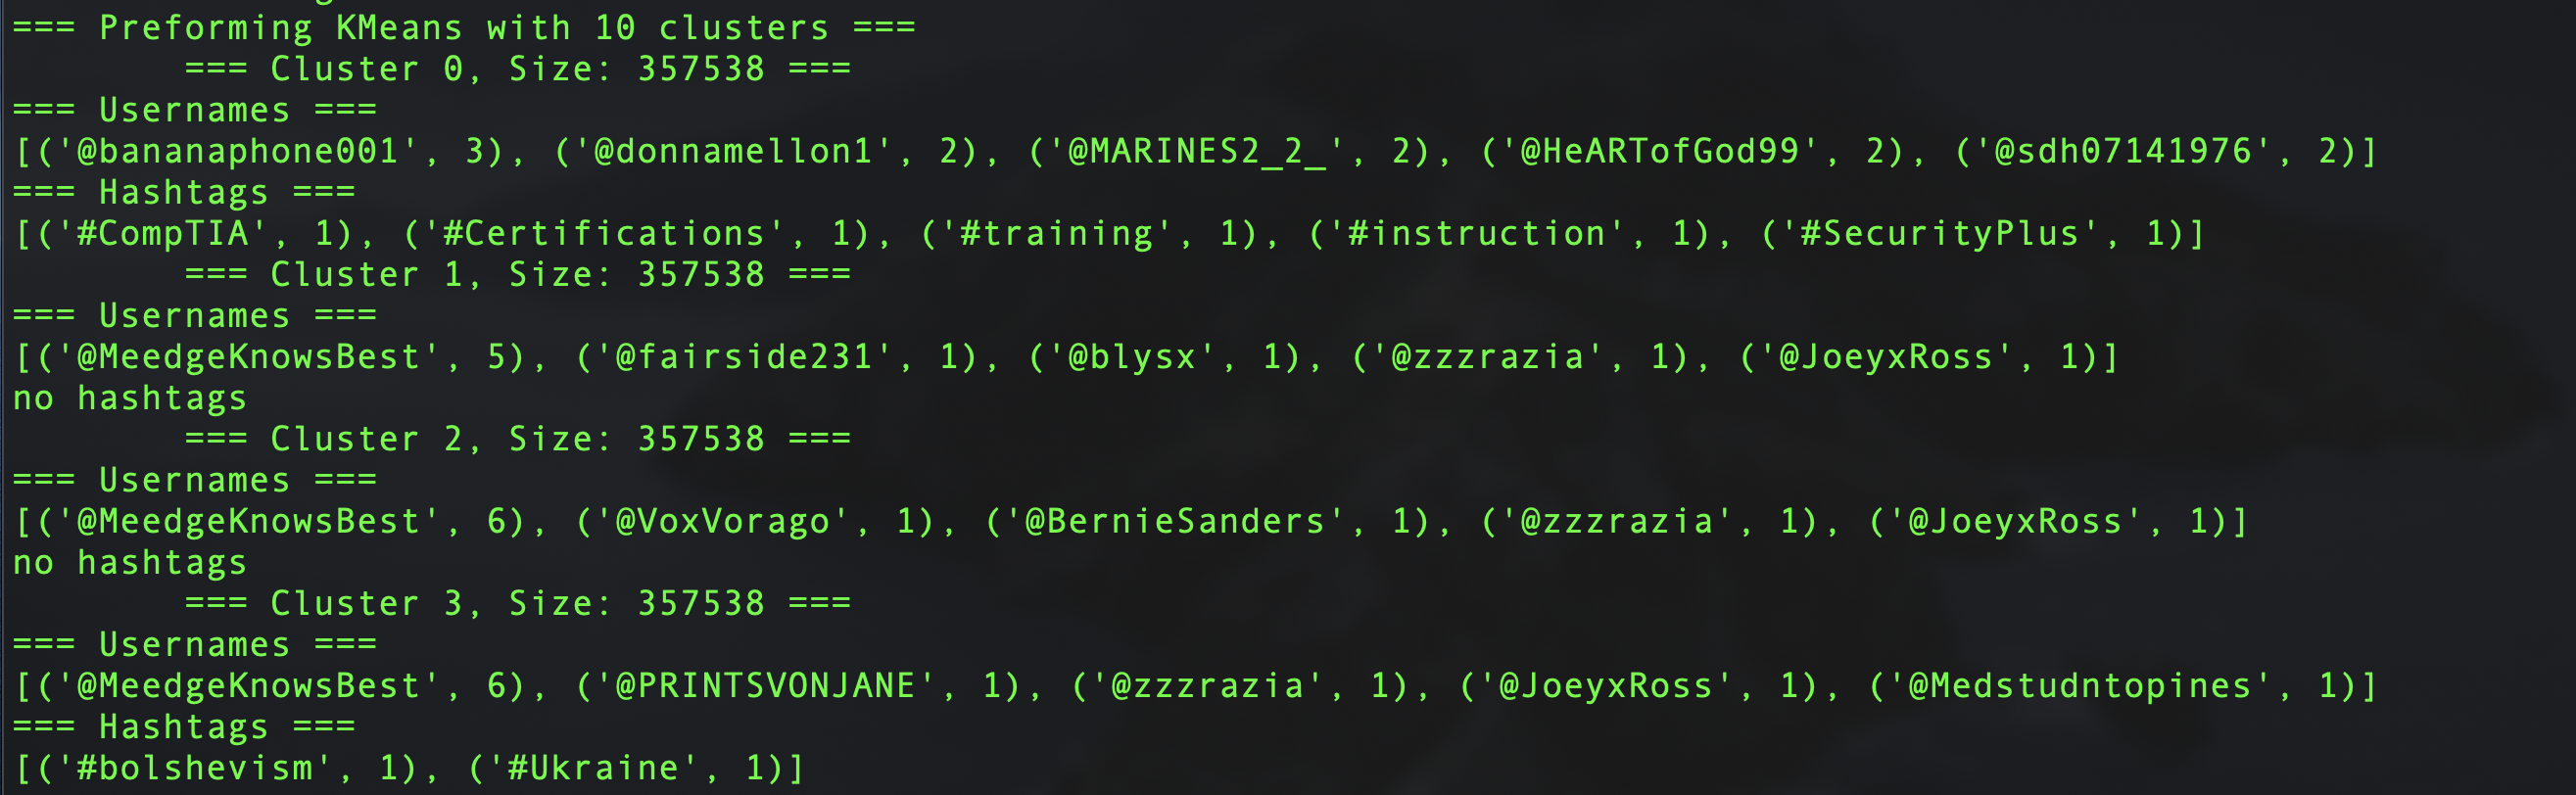
\includegraphics[width=\textwidth]{images/cluster_example.png} 

	\subsection*{Text grouping}
	
	I also wrote another script called \verb|cluster_text.py| to cluster the text alone and print out the top 10 terms, this however strips the \verb|@| and \verb|#| symbols.

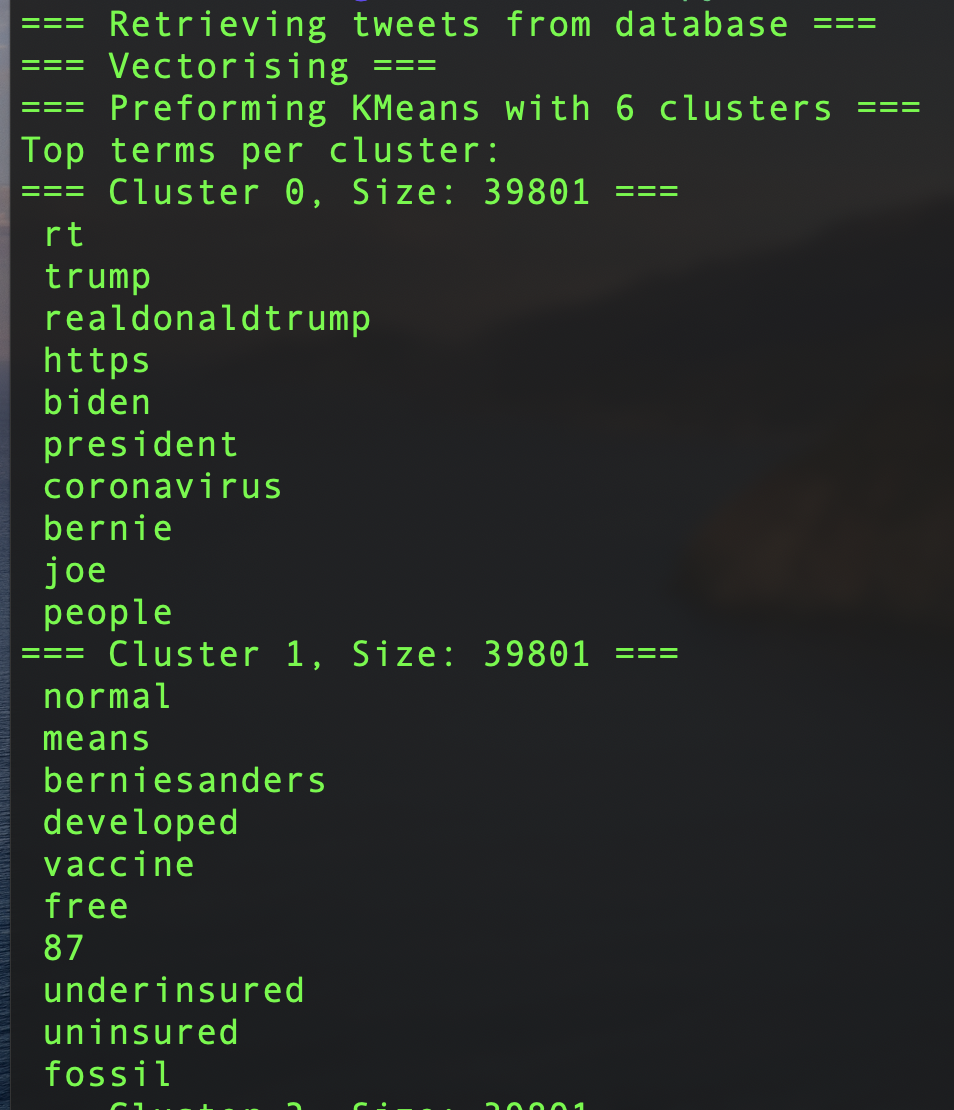
\includegraphics[scale=0.35]{images/words_cluster.png} 
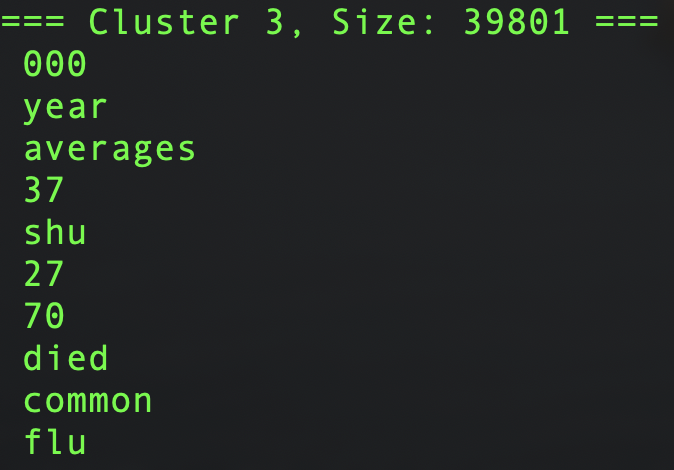
\includegraphics[scale=0.35]{images/virus_cluster.png} 

I choose to only use a sample of 50,000 tweet as it can take a long time to cluster using KMeans, I used 6 clusters as that gave some good clusters on the different candidates as well as one on the coronavirus. Again because I used KMeans, all the clusters were of equal sizes.

\section{Methods for constructing user interaction graphs}
\subsection*{a. Mentions, Replies, Retweets and Quote Tweets}
	Capturing and organising user interactions such as mentions, replies, retweets, and quote tweets is done by the \verb|user_interactions.py| script. I had a problem with indexing the nested json format of the mongoDB database so the script normalises the data taken in through pymongo (This can take some time!) before storing in a pandas dataframe. The initial dataframe is parsed to retrieve relevant information which is stored in another dataframe which is itself parsed using the \verb|get_interactions| function which contains lines which can be commented in and out to control which interactions are recorded. After the interactions are recorded, the networkx library is used to construct the graph with the nodes being users and the edges being interactions. I used a sample size of 10,000 tweets for each graph as the runtime increases exponentially for drawing the graphs, especially the mentions graph.
	
\subsection*{b. Hashtag co occurrence}	

	To capture hashtag co occurrence information I used a website \url{https://www.cortext.net} to generate maps of hashtags commonly used together by multiple users. In order to get the data in a format that was readable by the website I constructed a script \verb|get_hashtags.py| that would read in a raw tweet json collection from mongoDB and output a csv file\verb|hashtags.csv| containing one column filled with all hashtags from the entities filed of a tweet separated by spaces.
	
	
	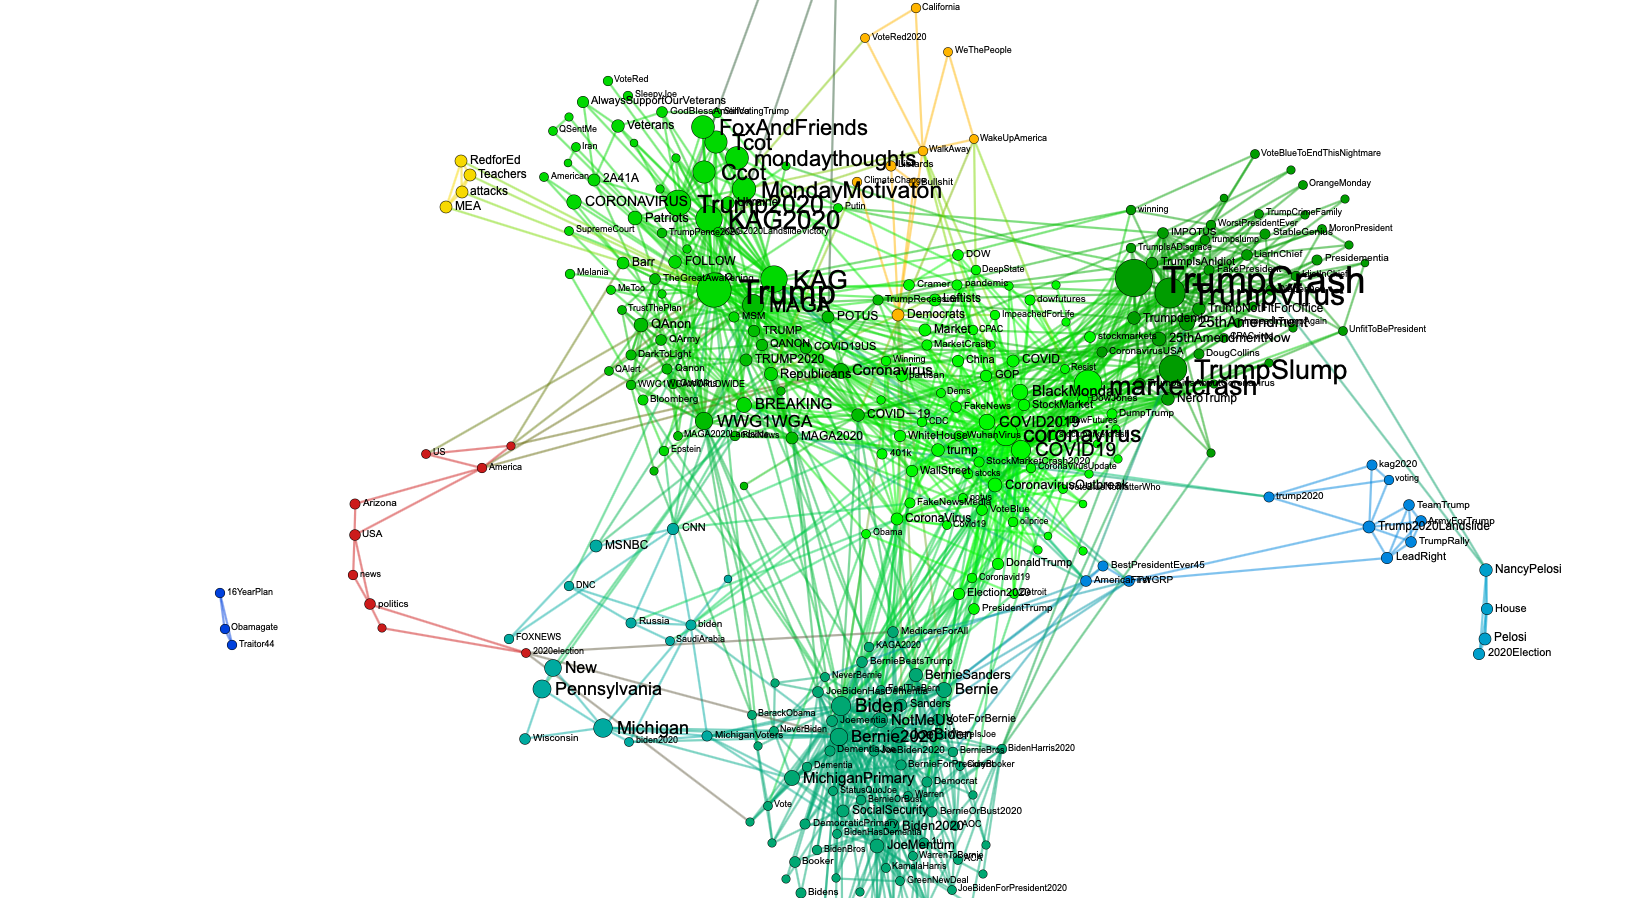
\includegraphics[width=\textwidth]{images/whole_hashtags_graph.png} 
	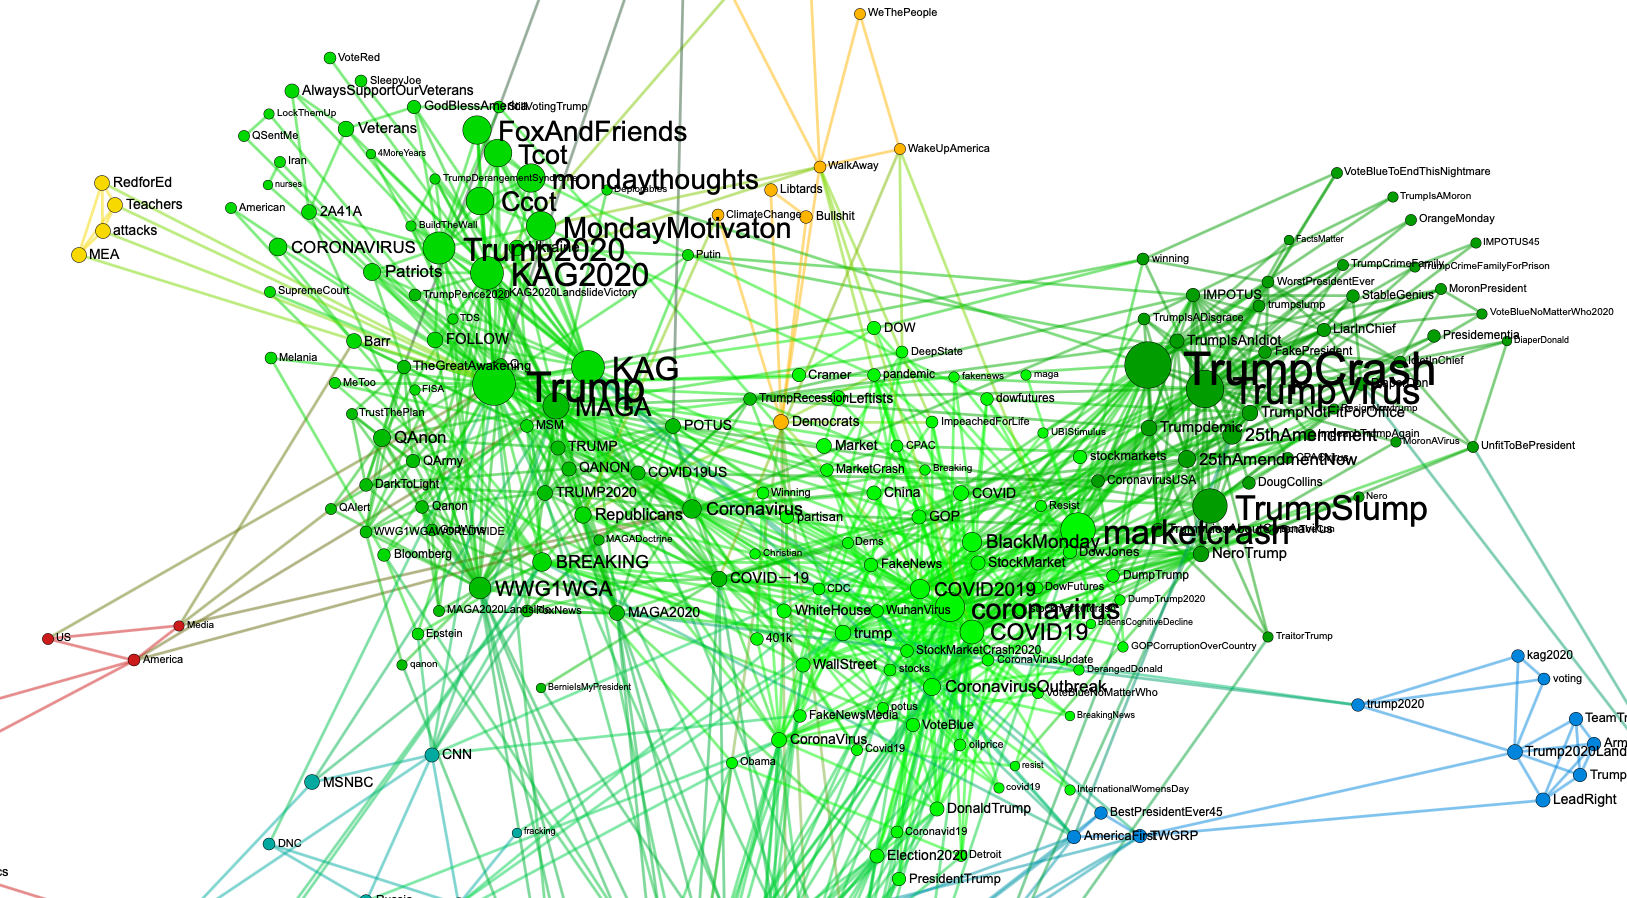
\includegraphics[width=\textwidth]{images/trump_hashtags.png}
	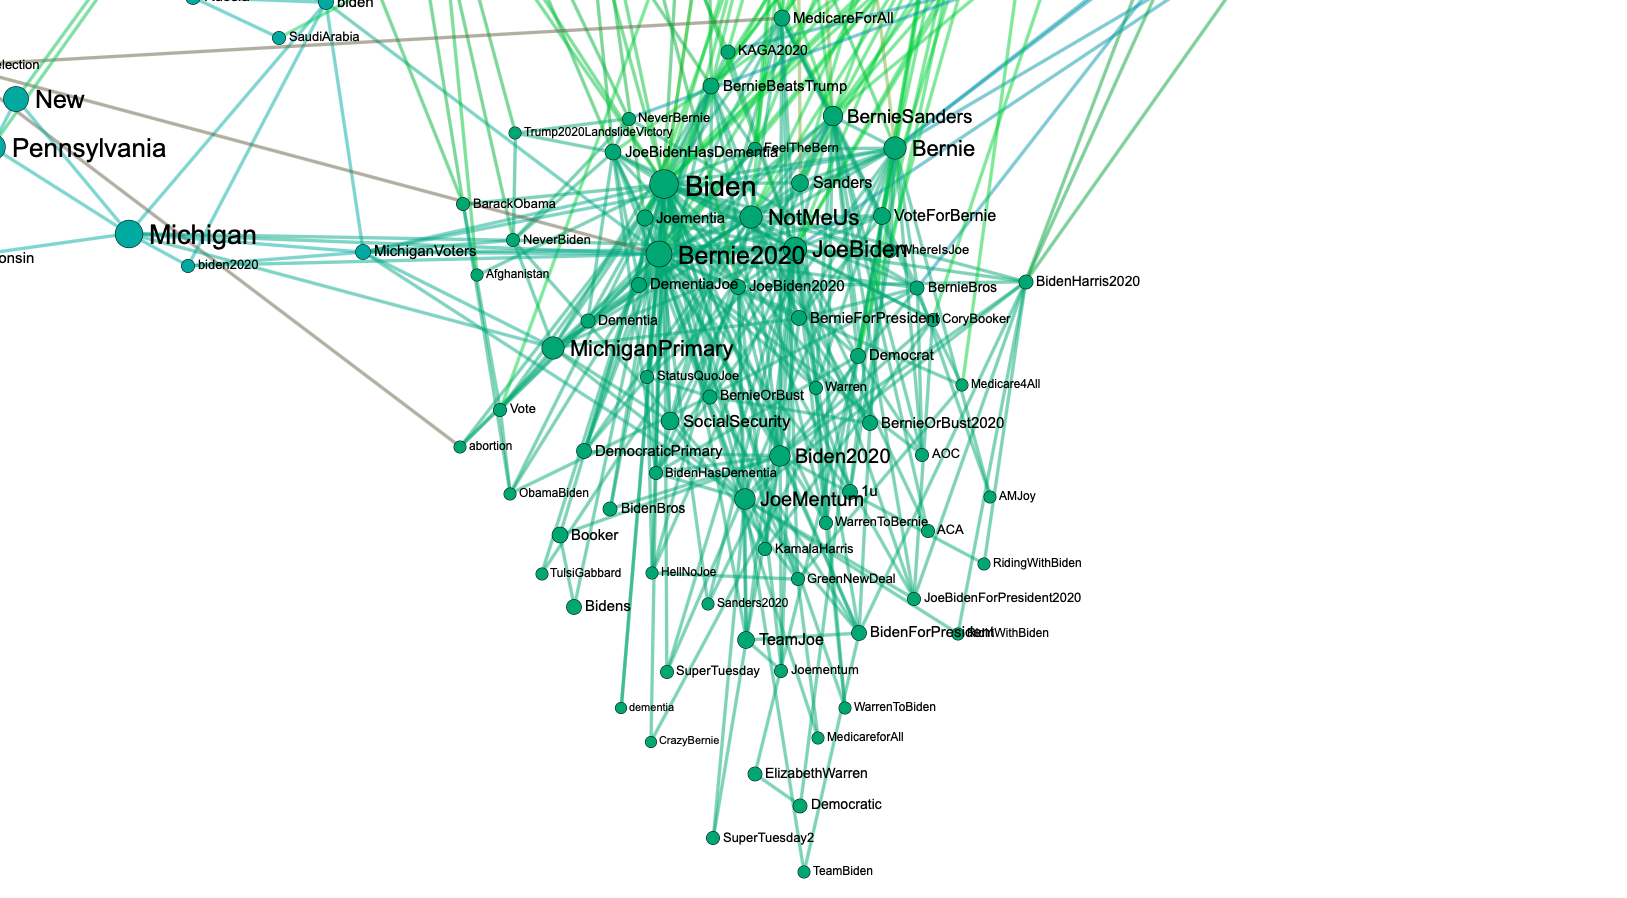
\includegraphics[width=\textwidth]{images/democrat_hashtags.png} 
	
	Here are screen shots from the hashtag graphs that show that the most popular hashtags used were in relation to Donald Trump. The graph seems to be similar in shape to that of the quotes and replies graphs seen below which leads me to suspect that the epicentres of the tries and triads in the graphs relate to a similar subject.
	
	
\section{Network analysis information}	

 	\subsection*{Mentions}
 	For the mentions graph with 7992 nodes and 7991 edges the average degree of the nodes was 2 yet the most frequent was 1.
 	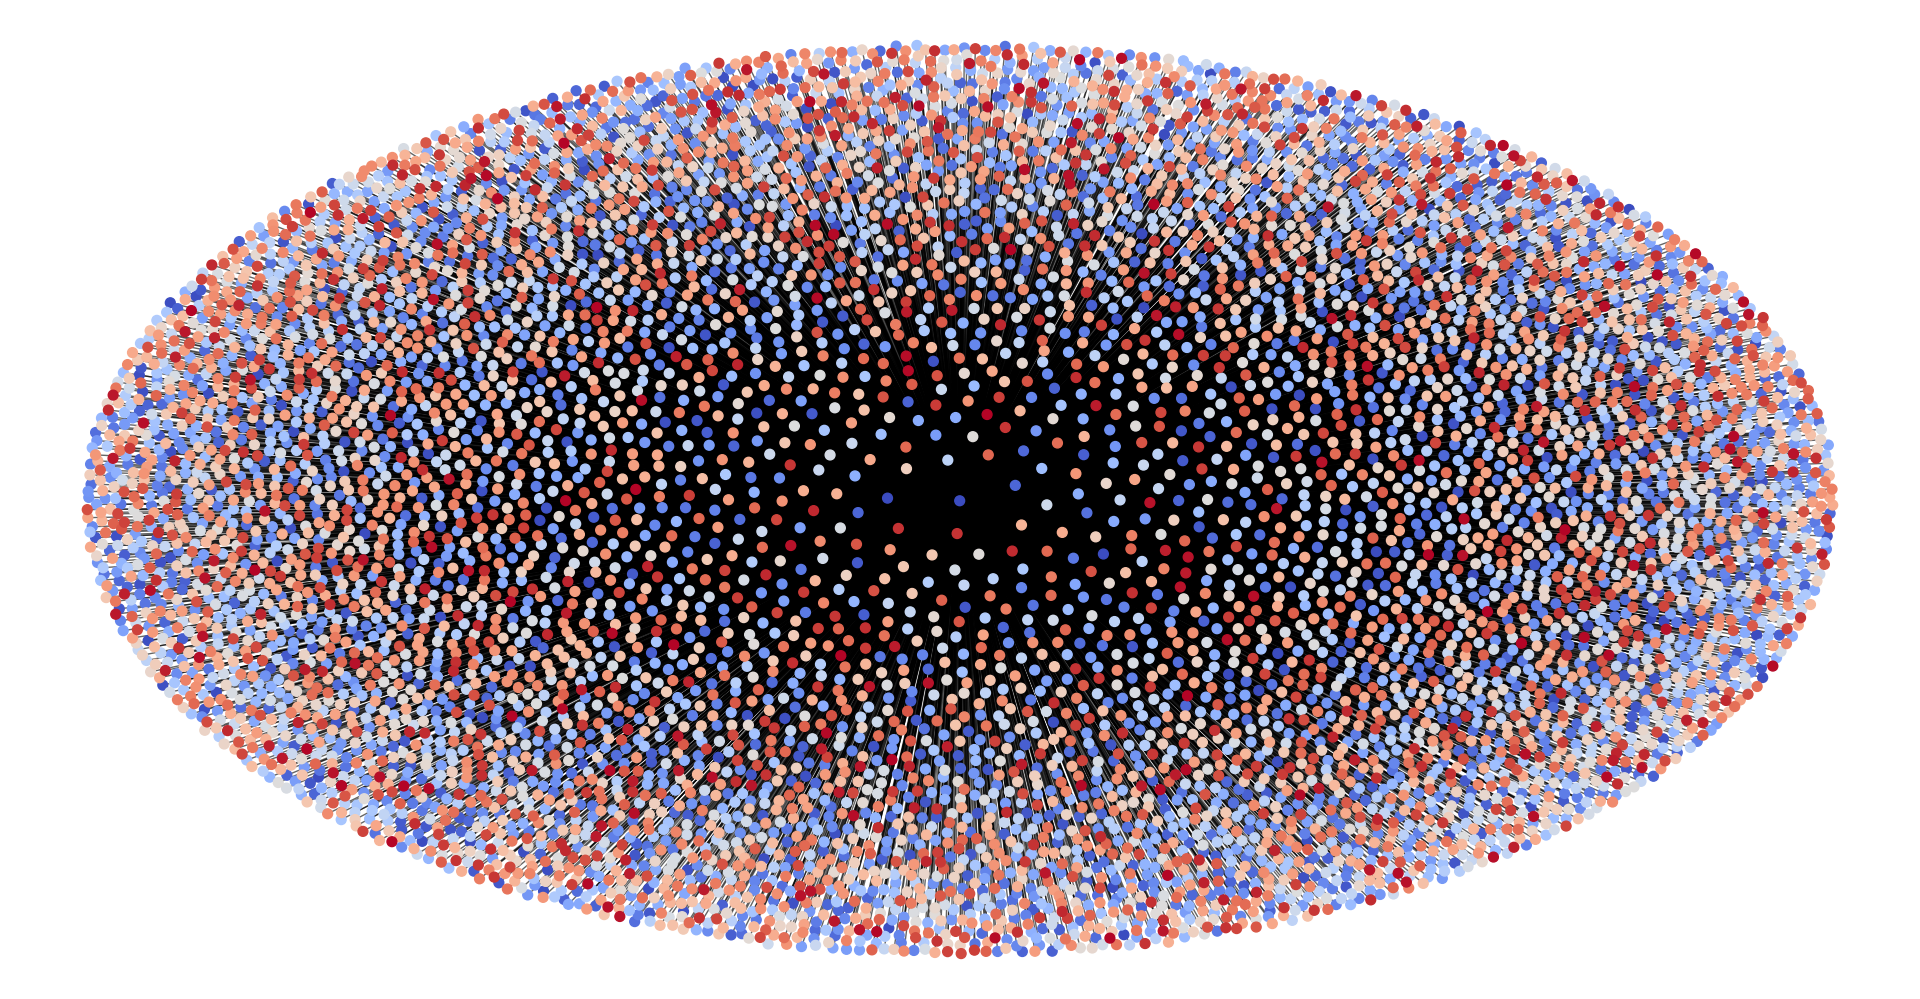
\includegraphics[width=\textwidth]{images/mentions_graph.png}
 	As can be seen from the graph it is clear that there is a central user being mentioned the most.
 	
 	
 	\subsection*{Retweets}
 	For the Retweets graph with 7872 nodes and 7008 edges the average degree of the nodes was 1.8 the most frequent was 1.
 	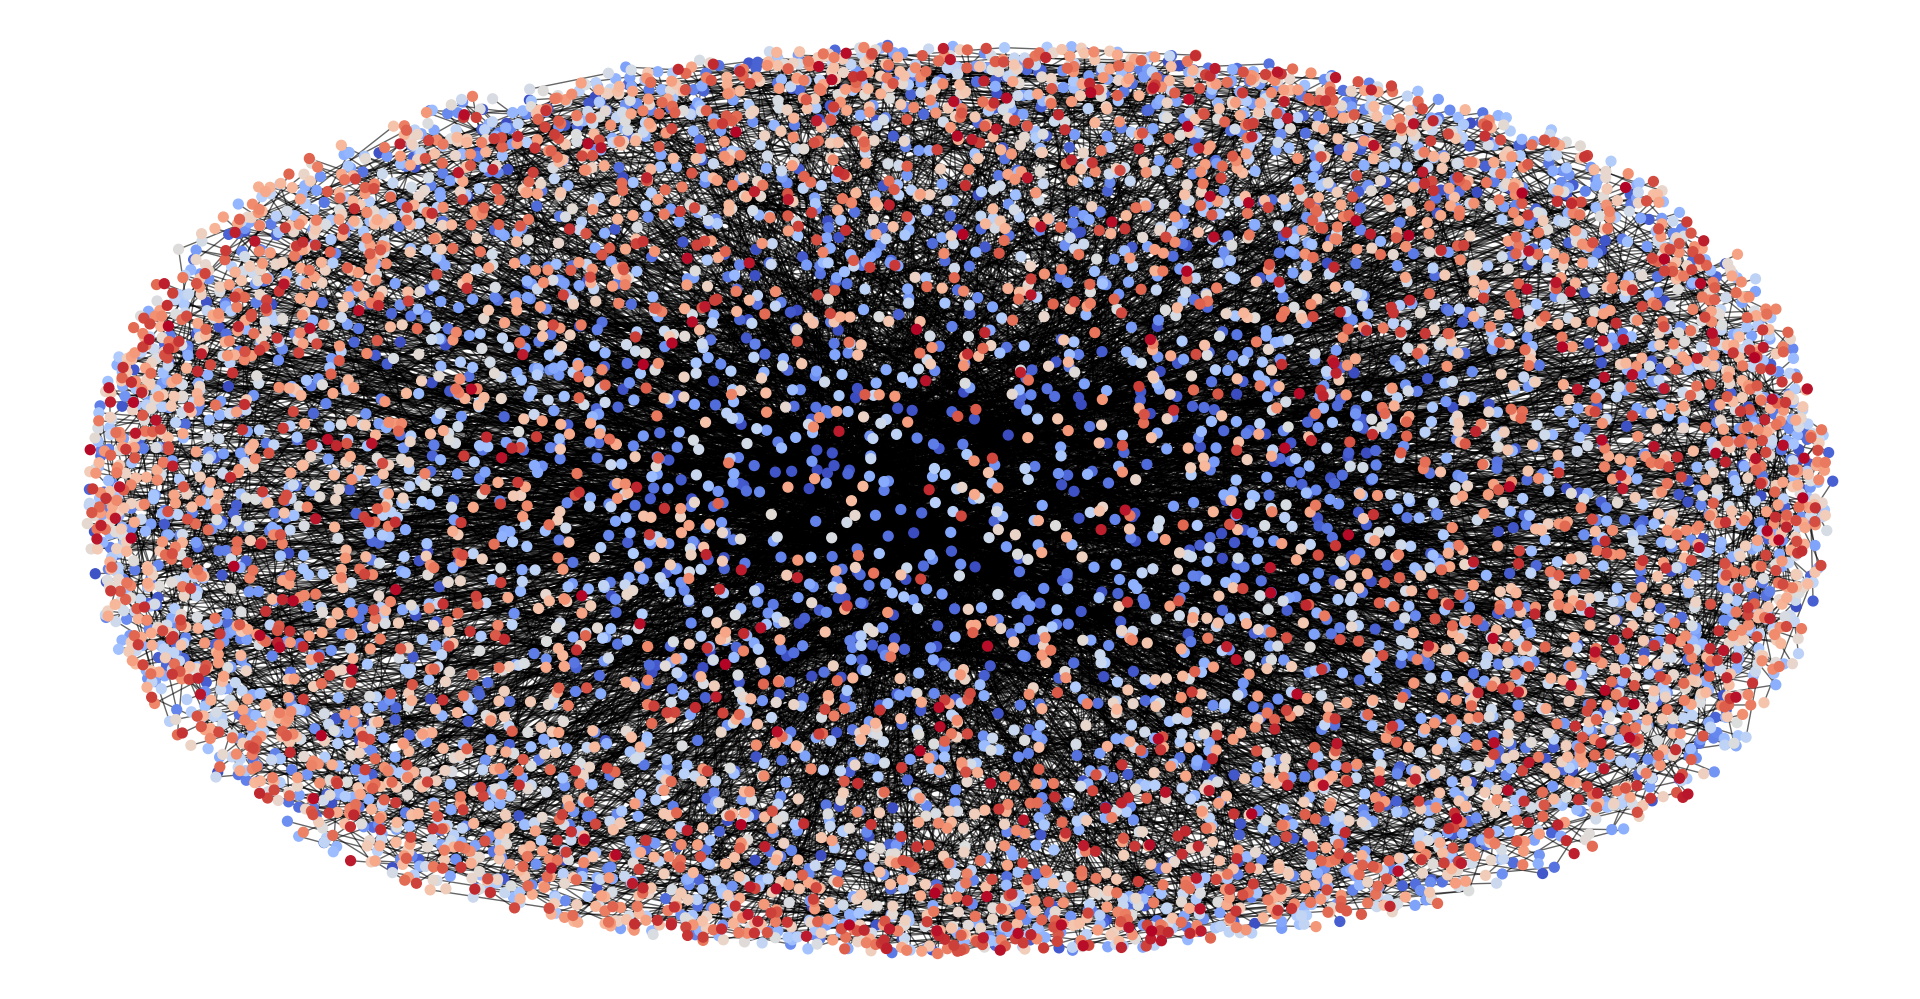
\includegraphics[width=\textwidth]{images/retweets_graph.png} 
 	This graph shows that there are many tweets being retweeted but in my data collection most are only retweeted by one user as the most frequent degree is 1
 	\subsection*{Replies}
	For the Replies graph with 2484 nodes and 1591 edges the average degree of the nodes was 1.3 the most frequent was 1.
 	 	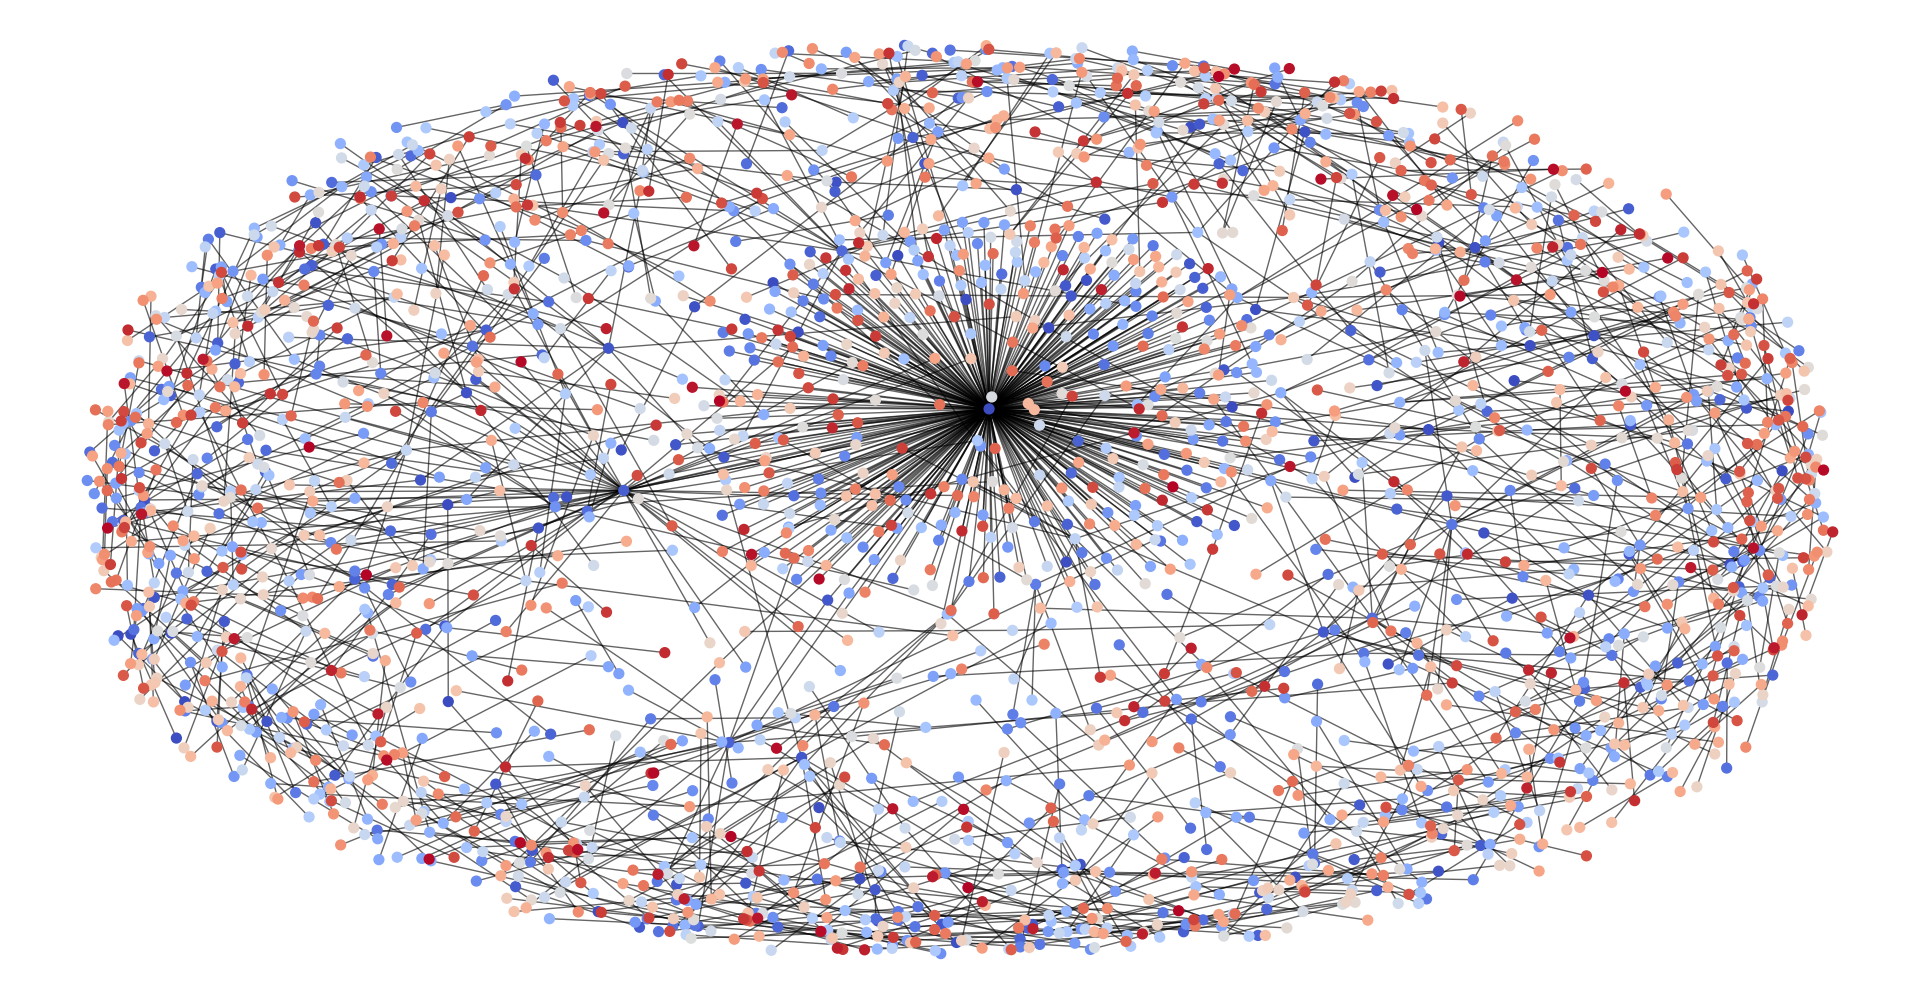
\includegraphics[width=\textwidth]{images/replies_graph.png} 
 	 	It can be seen from the graph that there is a clear tweet in the centre that was replied to the most.
 	\subsection*{Quotes}
	For the Quotes graph with 2340 nodes and 1769 edges the average degree of the nodes was 1.5 the most frequent was 1.
	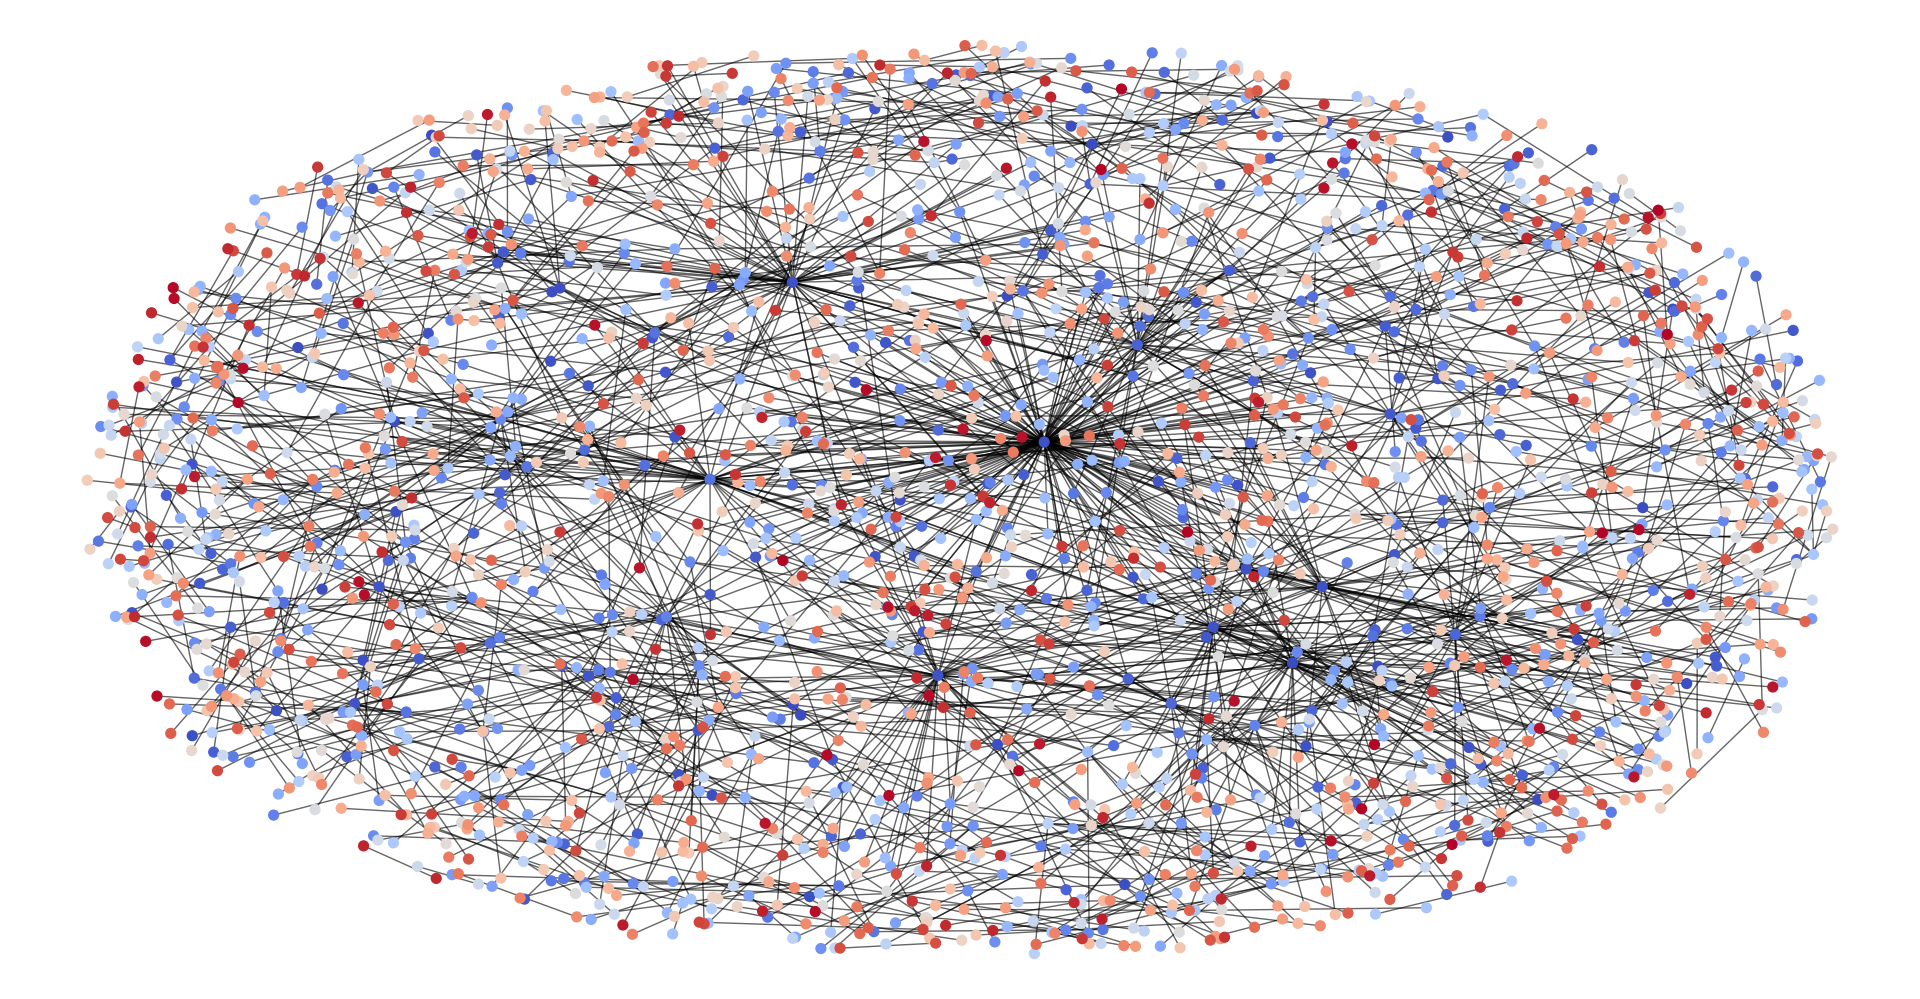
\includegraphics[width=\textwidth]{images/quotes_graph.png} 
	As can be seen from the graph few clear tweets that were quoted the most.

\section*{Sample Data}
	Sample data is provided in the \verb|all_tweets.json| file and must be imported into a local mongoDB database \verb|TwitterStream| and collection \verb|all_tweets| for the scripts of function correctly. Alternately new data can be collected by the \verb|get_twitter_data.py| script.

\end{document}